\documentclass[aps,prb,reprint,superscriptaddress,floatfix]{revtex4-2}
% Portable fallback: if revtex4-2 is unavailable, replace the line above with
%   \documentclass[twocolumn]{article}
% and the manuscript still compiles with the packages below.
\usepackage{amsmath,amssymb}
\usepackage{braket}
\usepackage{graphicx}
\usepackage{booktabs}
\usepackage[version=4]{mhchem}

\newcommand{\Hbar}{\bar{H}}
\newcommand{\op}[1]{\hat{#1}}
\newcommand{\ee}{\mathrm{e}}

\begin{document}

\title{Transcorrelated Mixed-Reference Spin-Flip
Configuration Interaction Singles (TC--MRSF-CIS):\\
Non-dynamical and dynamical correlation for excited states at
$\mathcal{O}(N^5)$}

\author{C.~H.~Choi}
\email[Corresponding author: ]{cheolho.choi@gmail.com}
\affiliation{Department of Chemistry, Kyungpook National University}
\author{S.~Ten-no}
\email[Corresponding author: ]{tenno@garnet.kobe-u.ac.jp}
\affiliation{Graduate School of System Informatics, Kobe University, Kobe 657-8501, Japan}

\date{\today}

\begin{abstract}
Mixed-reference spin-flip (MRSF) methods deliver spin-pure, multireference-quality
descriptions of ground and excited states---diradicals, bond dissociation,
doubly-excited states, and the correct topology of conical intersections,
including the $S_0/S_1$ seam---within a single-reference, configuration-interaction-singles
(CIS) cost. At the bare Hartree--Fock level, however, MRSF-CIS lacks dynamic
correlation and does not describe the electron--electron cusp, so excitation
energies are systematically biased and basis-set convergence is slow. We propose
\emph{transcorrelated} MRSF-CIS (TC--MRSF-CIS): the bare electronic Hamiltonian is
replaced by a non-Hermitian transcorrelated effective Hamiltonian
$\Hbar=\ee^{-\tau}H\,\ee^{\tau}$ that injects dynamic correlation and the
spin-resolved cusp directly into the operator, without a density functional and
without the double-counting problem that hampers transcorrelated Kohn--Sham theory.
We develop and compare two routes: the Boys--Handy~\cite{boys1969} Jastrow
transcorrelation, and Ten-no's projective transcorrelation
(pTC)~\cite{tenno2000,tenno2023}, whose F12-inspired generator dispenses with the
quadratic-in-correlator terms and converges, at second order, to the $V$-term of
explicitly-correlated MP2 (MP2-F12) at roughly half the cost. Both use the same
Slater geminal whose direct/exchange amplitudes satisfy the singlet \emph{and}
triplet first-order cusp conditions simultaneously, free of spin contamination,
matching the spin purity of the mixed reference. Because the correlator satisfies the singlet \emph{and} triplet
first-order cusp conditions simultaneously and is free of spin contamination, it
is uniquely matched to the spin purity of the mixed reference. We show that the
resulting method retains the $\mathcal{O}(N^5)$ (MP2-class) scaling of MRSF-CIS
provided the three-body term of $\Hbar$ (the only many-body term a two-body
correlator generates) is normal-ordered against the reference density and
density-fitted. The transcorrelated response matrix is non-Hermitian; we present
a general (non-symmetric) reduced-space eigensolver returning real eigenvalues
with biorthonormal left/right Ritz vectors, validated to reproduce the symmetric
limit to machine precision. Proof-of-concept calculations carried out with a
self-contained, package-free implementation establish the construction:
an exactly-solvable Hubbard dimer in which the transcorrelated mean-field
determinant recovers $100\%$ of the correlation energy and the non-Hermitian
solver returns the exact spectrum; and \ce{H2} dissociation from an ROHF
reference, where the genuine first-quantized $\Hbar$---built from Ten-no's
cusp-fixed geminal and constituting the \emph{complete} transcorrelated
Hamiltonian for a two-electron system---pulls bare MRSF-CIS essentially onto the
in-basis FCI across the whole curve and, as a transcorrelated FCI, drives the
finite-basis energy down to the exact Kolos--Wolniewicz limit, recovering the
basis-set incompleteness. Every bare energy is reproduced by an independent
\textsc{PySCF} calculation to all printed digits, the transcorrelated integrals
are certified to $\sim\!10^{-12}$ against analytic and operator-identity targets,
and the transcorrelated spectrum is exactly real. We argue that
TC--MRSF-CIS occupies a distinctive niche relative to ADC(2): equal
$\mathcal{O}(N^5)$ scaling and comparable dynamic correlation, but with the
non-dynamical correlation and correct conical-intersection topology that
single-reference perturbation theories lack.
\end{abstract}

\maketitle

\section{Introduction}

The accurate and affordable description of electronically excited states remains
a central challenge of quantum chemistry. The difficulty is sharpest where two
qualitatively different kinds of electron correlation must be captured at once.
\emph{Non-dynamical} (static) correlation arises when several electronic
configurations become near-degenerate---in diradicals, homolytic bond
dissociation, doubly-excited states, and at the conical intersections that funnel
nonadiabatic relaxation---so that a single Slater determinant is already
qualitatively wrong. \emph{Dynamic} correlation is the short-range, cusp-driven
mutual avoidance of electrons that no finite sum of smooth orbital products
reproduces, and that converges only slowly with the size of the one-particle
basis. Methods that treat one kind of correlation well typically treat the other
poorly; an approach that supplies both at a modest, $\mathcal{O}(N^5)$ cost would
fill a persistent gap.

Linear-response time-dependent density functional theory (TDDFT) is the workhorse
for medium and large systems, but within the ubiquitous adiabatic approximation
its exchange--correlation kernel is frequency-independent: genuinely
doubly-excited states are therefore absent from the linear-response spectrum, and
the $S_0/S_1$ intersection seam acquires the wrong dimensionality, because a
same-symmetry crossing between the ground and first excited state cannot be
represented when only one of the two carries an explicit response. Single-reference
wavefunction response methods such as ADC(2)~\cite{schirmer1982,dreuw2015} and
CC2 add rigorous dynamic correlation at $\mathcal{O}(N^5)$, but they are built on
a M{\o}ller--Plesset ground state and inherit its divergence wherever the
reference determinant ceases to dominate---that is, in precisely the
multireference regions of greatest interest. Genuinely multireference treatments
(CASPT2, MRCI, NEVPT2) describe both correlation types accurately but carry a
steep computational cost and the practical burden of selecting and balancing an
active space along a reaction coordinate.

The spin-flip (SF) family~\cite{krylov2001} offers a single-reference route to
multireference targets. A high-spin reference---typically the $M_s=+1$ component
of a triplet---is chosen precisely because it remains well described by a single
determinant even where the low-spin states are strongly correlated; the target
$M_s=0$ states are then generated by spin-flipping ($\alpha\!\to\!\beta$) single
excitations, so that the closed- and open-shell singlets and the $M_s=0$ triplet
all appear on an equal footing within a problem no larger than CIS. The weakness
of the original construction is spin contamination: the set of spin-flipping
single excitations out of one high-spin determinant is not closed under
$\op{S}^2$, so the computed states emerge as mixtures of spin multiplicities.
Spin-complete and restricted-active-space variants restore purity by enlarging
the excitation manifold. The mixed-reference spin-flip
(MRSF)~\cite{lee2018,horbatenko2021} construction instead restores spin
completeness compactly, by forming the response from \emph{both} the $M_s=+1$ and
$M_s=-1$ components of the triplet reference. The combination yields spin-pure
singlet and triplet states, a ground state $S_0$ recovered as one of the response
roots on the same footing as the excited states, and the correct branching-space
dimensionality at conical intersections---all retained at CIS cost.

What MRSF-CIS lacks at the bare Hartree--Fock level is dynamic correlation and any
description of the interelectronic cusp---the derivative discontinuity that the
exact wavefunction develops as two electrons coalesce and that no smooth product
of one-particle functions can reproduce. Its omission is the common origin of two
deficiencies: a systematic bias in MRSF-CIS excitation energies, and the slow,
$\mathcal{O}(L^{-3})$ convergence of those energies with the maximum angular
momentum $L$ of the one-particle basis. In practice the missing correlation is
restored by a density functional (MRSF-TDDFT), which is remarkably successful but
introduces a dependence on the chosen functional and, more fundamentally, a
double-counting ambiguity should one later wish to add explicit correlation on top
of an exchange--correlation functional that already models it implicitly.

Here we pursue a different, functional-free route through transcorrelation. In the
Boys--Handy transcorrelated method~\cite{boys1969}, the Hamiltonian is
similarity-transformed by a fixed correlation (Jastrow) factor,
$\Hbar=\ee^{-\tau}H\,\ee^{\tau}$, so that explicit electron correlation is built
into the \emph{operator} rather than carried by an ever-larger expansion of the
wavefunction. Because the cusp is imposed analytically through $\tau$, even a
compact---or mean-field---wavefunction evaluated with $\Hbar$ recovers correlation
that the same wavefunction misses under the bare $H$, and basis-set convergence is
accelerated by orders of magnitude. Long confined to specialized applications, TC
has lately undergone a strong revival, driven by accurate correlators and by the
pairing of $\Hbar$ with full-configuration-interaction quantum Monte Carlo,
density-matrix renormalization group, and coupled-cluster solvers. The
correlator we adopt is Ten-no's explicitly-correlated geminal~\cite{tenno2000,tenno2023},
which is especially well matched to the present aim: it is non-Hermitian, free of
spin contamination, and its amplitudes are fixed analytically by the first-order
coalescence-cusp conditions for both antiparallel-spin (singlet) and
parallel-spin (triplet) pairs simultaneously. These are exactly the properties
demanded by a spin-pure mixed reference.

We therefore propose TC--MRSF-CIS, in which the MRSF-CIS response is built from
Ten-no's non-Hermitian transcorrelated Hamiltonian---the Boys--Handy similarity
transform of $H$ by Ten-no's cusp-fixed geminal. The construction adds
dynamic correlation and correct cusp behaviour to MRSF-CIS, dispenses with the
exchange--correlation functional and its double-counting ambiguity, retains the
$\mathcal{O}(N^5)$ scaling of MRSF-CIS, and---by design---matches the
spin-resolved cusp of TC to the spin purity of the mixed reference. The remainder
of this paper develops the working equations (Sec.~\ref{sec:theory}), isolates and
validates the single new numerical kernel that the non-Hermiticity requires---a
reduced-space eigensolver for a non-symmetric matrix
(Sec.~\ref{sec:eigensolver})---and demonstrates the spin-flip construction and the
correlation-recovery mechanism on exactly controllable systems
(Sec.~\ref{sec:results}).

\section{Theory}\label{sec:theory}

\subsection{MRSF-CIS}

Let $\op{a}^\dagger_{p\sigma}$ and $\op{a}_{p\sigma}$ denote creation and
annihilation operators for spatial orbital $p$ and spin $\sigma$, and partition
the orbitals of a high-spin restricted-open-shell Hartree--Fock (ROHF) triplet
into a doubly-occupied (closed) set $\{i,j,\dots\}$, two singly-occupied frontier
(open) orbitals $\{O_1,O_2\}$, and a virtual set $\{a,b,\dots\}$. The reference
exists as two degenerate $M_s=\pm1$ determinants,
\begin{equation}
\ket{T_{+}}=\op{a}^\dagger_{O_1\alpha}\op{a}^\dagger_{O_2\alpha}\ket{\mathrm{core}},
\qquad
\ket{T_{-}}=\op{a}^\dagger_{O_1\beta}\op{a}^\dagger_{O_2\beta}\ket{\mathrm{core}},
\end{equation}
which differ only in the spin of the two open-shell electrons. Single-reference
spin-flip would build the $M_s=0$ manifold from $\ket{T_{+}}$ alone; MRSF instead
forms it from \emph{both} components, so that the spin-flip excitations missing
from one reference are furnished by the other,
\begin{equation}
\ket{\Psi_I}=\sum_{ia}\, c^{I,+}_{ia}\,
\op{a}^\dagger_{a\beta}\op{a}_{i\alpha}\,\ket{T_{+}}
+\sum_{ia}\, c^{I,-}_{ia}\,
\op{a}^\dagger_{a\alpha}\op{a}_{i\beta}\,\ket{T_{-}}.
\label{eq:mrsfstate}
\end{equation}
Within the frontier (open-shell) block these spin-flipping single excitations are
supplemented by the small set of correction configurations that render the
combined manifold an eigenfunction of $\op{S}^2$, while the closed$\to$open and
open$\to$virtual classes deliver the ground state $S_0$ as a response root
alongside the excited states. Diagonalizing the spin-adapted, mixed-reference
Hamiltonian over this manifold gives the Tamm--Dancoff (CIS-like) Hermitian
eigenproblem
\begin{equation}
\mathbf{A}\,\mathbf{c}^I=\omega_I\,\mathbf{c}^I,
\qquad \mathbf{A}=\mathbf{A}^{\mathsf{T}},
\label{eq:mrsf}
\end{equation}
solved by a symmetric Davidson iteration. Each matrix--vector product
$\mathbf{A}\mathbf{c}$ is a Fock-like contraction of two-electron integrals with
the trial vector and costs $\mathcal{O}(N^4)$ per iteration; the matrix itself is
never formed explicitly.

We consider two complementary, non-unitary transcorrelations that both build the
electron--electron cusp into the operator rather than the wavefunction, and both
yield a non-Hermitian $\Hbar$ that feeds the MRSF response identically: the
\emph{Boys--Handy} Jastrow transcorrelation, and \emph{Ten-no's projective
transcorrelation} (pTC). They share the cusp-fixed Slater geminal but differ in
how the correlator acts and which terms survive; we present both and compare them
numerically in Sec.~\ref{sec:results}.

\subsection{Boys--Handy transcorrelation}

The transcorrelated Hamiltonian is the non-unitary Boys--Handy similarity
transform~\cite{boys1969}
\begin{equation}
\Hbar=\ee^{-\tau}\,H\,\ee^{\tau},
\label{eq:tc}
\end{equation}
in which the correlator is a symmetric, real, two-body Jastrow operator
$\tau=\sum_{i<j}u(r_{ij})$ built from a fixed correlation factor $u$ that encodes
the interelectronic cusp; in the F12 spirit $u$ is a Slater-type geminal (or its
Gaussian expansion) whose short-range slope is set analytically rather than
variationally optimized. The Baker--Campbell--Hausdorff identity gives
\begin{equation}
\Hbar=H+[H,\tau]+\tfrac12\big[[H,\tau],\tau\big]+\cdots .
\label{eq:bch}
\end{equation}
Because $\tau$ is multiplicative it commutes with the electron--electron and
electron--nucleus potentials; only the kinetic operator $\op{T}$ fails to commute,
so the series~\eqref{eq:bch} truncates \emph{exactly} at the double commutator.
Evaluating the commutators yields the closed form
\begin{equation}
\Hbar=H-\sum_i\Big[\tfrac12\nabla_i^2\tau
+(\nabla_i\tau)\!\cdot\!\nabla_i
+\tfrac12(\nabla_i\tau)^2\Big].
\label{eq:hbar-explicit}
\end{equation}
The scalar $\nabla_i^2\tau$ term renormalizes the one- and two-body potential; the
$(\nabla_i\tau)\!\cdot\!\nabla_i$ term is a non-Hermitian first-derivative
(``drift'') coupling and is the sole source of the non-Hermiticity; and the
$(\nabla_i\tau)^2$ term, through the cross terms $j\neq k$ in
$\nabla_i\tau=\sum_j\nabla_i u(r_{ij})$, contributes a two-body piece together
with a genuine three-body piece. For a two-body correlator the series terminates
\emph{exactly} at this three-body term---there is no four-body contribution. The
amplitudes of $u$ are fixed by Ten-no's explicitly-correlated
prescription~\cite{tenno2000,tenno2023}: the two first-order coalescence-cusp
conditions---the $\tfrac12$ cusp of an antiparallel-spin (singlet) pair and the
$\tfrac14$ cusp of a parallel-spin (triplet) pair---are imposed simultaneously,
with no variational optimization, leaving $\Hbar$ free of spin contamination. The
price of this explicit, functional-free correlation is that $\Hbar$ is
\emph{non-Hermitian}. The cross terms also generate the genuine three-body
operator $-\tfrac12\sum_i\sum_{j\neq k}(\nabla_i u_{ij})\!\cdot\!(\nabla_i u_{ik})$,
which for the $\mathcal{O}(N^5)$ target is normal-ordered against the reference
into effective one- and two-body operators (the three-body remainder is neglected,
as is standard in transcorrelated theory).

\subsection{Ten-no's projective transcorrelation (pTC)}
\label{sec:ptc}

The Jastrow form above is variationally unbounded and, in a finite basis, mixes
the in-basis and out-of-basis correlation. Ten-no's projective transcorrelation
(pTC)~\cite{tenno2023} removes both issues by recasting the similarity transform in
the F12 framework. Rather than a multiplicative factor acting in the full space,
the generator excites an occupied electron pair $(rs)$ into the space orthogonal
to the orbital basis,
\begin{equation}
\op{G}=\tfrac12\,\big\langle\kappa\lambda\big|\,\op{Q}_{12}\,\op{R}_{12}\,\big|rs\big\rangle\,
\op{E}^{\kappa\lambda}_{rs},
\label{eq:gen}
\end{equation}
where $\op{Q}_{12}=(1-\op{P}_1\op{P}_2)(1-\op{O}_1)(1-\op{O}_2)$ projects onto the
complement of the orbital-basis pairs ($\op{P}$) and the occupied space ($\op{O}$),
and the rational generator under the SP (fixed-amplitude) ansatz is
\begin{equation}
\op{R}_{12}=f(r_{12})\Big(\tfrac38+\tfrac18\,\op{P}_{12}\Big),\qquad
f(r_{12})=-\tfrac1\gamma\,\ee^{-\gamma r_{12}},
\label{eq:sp}
\end{equation}
with $\op{P}_{12}$ the spatial permutation. The direct ($\tfrac38$) and exchange
($\tfrac18$) coefficients satisfy the antiparallel ($\tfrac12$) and parallel
($\tfrac14$) first-order cusp conditions simultaneously. The pTC Hamiltonian
$\Hbar_{\mathrm{pTC}}=\mathcal{B}\{\ee^{-\op{G}}H\,\ee^{\op{G}}\}$, with
$\mathcal{B}\{\cdot\}$ the second-quantized representation within the orbital basis,
terminates formally at four-body interactions; the single contractions through the
complementary projector decay rapidly with basis size, so in practice
\begin{equation}
\Hbar_{\mathrm{pTC}}\approx H+\op{H}_{2h}+\op{H}_{2w}+\op{H}_{3l}.
\label{eq:hptc}
\end{equation}
Two features distinguish pTC from the Jastrow form. First, because $\op{G}$ acts
into the complement, the quadratic-in-$f$ operators $f^2(r_{12})$ and
$\nabla f\!\cdot\!\nabla f$---the source of the costly $B$- and $X$-intermediates in
conventional F12, and the $(\nabla\tau)^2$ term in Boys--Handy---\emph{do not
appear}. Second, the kinetic commutator regularizes the Coulomb singularity
analytically,
\begin{equation}
(\op{t}_1+\op{t}_2)\,\op{R}_{12}\,\ket{rs}=\big\{-r_{12}^{-1}+\mathcal{O}(r_{12}^0)\big\}\ket{rs},
\label{eq:reg}
\end{equation}
for both the singlet ($r{+}s$) and triplet ($r{-}s$) channels. At second order pTC
is equivalent to the $V$-term of explicitly-correlated MP2,
$E_{\mathrm{pTC}(2)}\approx E_{\mathrm{MP2}}+V$, so it inherits the rapid
basis-set convergence of MP2-F12 at roughly half the cost (no $B$-term integrals),
while remaining a genuine transcorrelation that dresses $\Hbar$ for the MRSF
response. Like the Jastrow form, $\Hbar_{\mathrm{pTC}}$ is non-Hermitian; the
complementary space is spanned in practice by a Gaussian complementary auxiliary
basis (CABS).

\subsection{Transcorrelated MRSF-CIS}

Replacing $H$ by $\Hbar$ in the MRSF-CIS matrix build of Eq.~\eqref{eq:mrsf}
yields the transcorrelated response matrix $\bar{\mathbf{A}}$. Its elements are
the same spin-flip configuration couplings as before, but now evaluated with the
effective one-, two-, and normal-ordered higher-body integrals of $\Hbar$; the
non-Hermitian drift term of Eq.~\eqref{eq:hbar-explicit} makes $\bar{\mathbf{A}}$
non-symmetric, $\bar{\mathbf{A}}\neq\bar{\mathbf{A}}^{\mathsf{T}}$. The eigenproblem
therefore splits into a right and a left problem,
\begin{equation}
\bar{\mathbf{A}}\,\mathbf{c}^I_{\!R}=\omega_I\,\mathbf{c}^I_{\!R},
\qquad
\bar{\mathbf{A}}^{\mathsf{T}}\,\mathbf{c}^I_{\!L}=\omega_I\,\mathbf{c}^I_{\!L},
\label{eq:tcmrsf}
\end{equation}
with distinct right and left eigenvectors obeying the biorthonormality condition
$\mathbf{c}^{I}_{\!L}\!\cdot\mathbf{c}^{J}_{\!R}=\delta_{IJ}$. A similarity
transform preserves the spectrum of the parent operator, so for every bound state
$\bar{\mathbf{A}}$ shares the real eigenvalues of its Hermitian limit; an
eigenvalue acquiring an imaginary part signals a breakdown of the transform---an
over-strong or poorly conditioned correlator---and is monitored as a numerical
diagnostic.

Crucially, everything that makes MRSF-CIS attractive---the mixed-reference spin
completeness, $S_0$ obtained as a response root, and the correct
conical-intersection topology---is left intact, because the reference and the
spin-flip excitation manifold are unchanged. What changes is only the operator
contracted inside the matrix build and, as a consequence, the symmetry of the
eigenproblem, which is handled by the solver of Sec.~\ref{sec:eigensolver}.

\subsection{Spin-resolved cusp and the choice of reference}

The cusp condition is spin-dependent. A spin-contaminated SF-CIS state, being a
mixture of singlet and triplet, satisfies neither the singlet nor the triplet
cusp cleanly, so a transcorrelation built for a definite spin state is applied to
an indefinite-spin object. The mixed-reference spin purity of MRSF removes this
mismatch: each state has a well-defined spin and therefore a well-defined cusp
that coincides with what TC corrects. This is the central reason MRSF, rather
than single-reference SF-CIS, is the appropriate substrate for
transcorrelation.

\subsection{Scaling and the higher-body terms}

The non-Hermitian eigenproblem~\eqref{eq:tcmrsf} is solved by a general
(non-symmetric) Davidson iteration of the same $\mathcal{O}(N^4)$/iteration cost
as the symmetric one; carrying left and right vectors increases the prefactor but
not the order. The rate-limiting step is the construction of $\Hbar$. Its genuine
three-body term (the only many-body operator a two-body correlator generates) is
never materialized: it is normal-ordered against the ROHF reference one-particle
density, folding its dominant contribution into effective one- and two-body
integrals, and the correlation factor is density-fitted (resolution of the
identity). With this treatment the $\Hbar$ build is $\mathcal{O}(N^5)$, consistent
with the cost of explicitly-correlated MP2-F12~\cite{tenno2023}. The explicit
three-body integral would be $\mathcal{O}(N^6)$; the normal-ordering/density-fitting
discipline is therefore essential and is the single design decision that keeps the
method at MP2 scaling. Sub-$N^5$ scaling is
in principle accessible because the correlation factor is short-ranged, via
local/pair-natural-orbital or tensor-hypercontraction techniques, but these are
deferred optimizations.

The final scaling is summarized as follows: ROHF reference, $\mathcal{O}(N^4)$;
integral transformation, $\mathcal{O}(N^5)$; $\Hbar$ build (normal-ordered,
density-fitted), $\mathcal{O}(N^5)$ (rate limiting); non-Hermitian Davidson,
$\mathcal{O}(N^4)$/iteration. Thus TC--MRSF-CIS is an $\mathcal{O}(N^5)$,
MP2-class method.

\section{Non-Hermitian reduced eigensolver}\label{sec:eigensolver}

The reduced-space (Davidson subspace) diagonalization is the one genuinely new
numerical kernel. Given a non-symmetric reduced matrix $\mathbf{A}_r$ we compute
the right and left eigenvectors in a single DGEEV pass, sort the (real) bound-state
eigenvalues, and rescale so that $\mathbf{c}_L^I\!\cdot\mathbf{c}_R^I=1$. With the
transcorrelation switched off ($\tau=0$), $\mathbf{A}_r$ is symmetric and the
kernel reproduces the symmetric solver to machine precision---the acceptance gate
for all of the non-Hermitian infrastructure. In our reference implementation this
gate is met at $\max|\Delta\omega|\sim7\times10^{-15}$~Ha, and a non-symmetric
test matrix is solved with right/left residuals and biorthonormality error of
order $10^{-14}$.

\section{Proof-of-concept results}\label{sec:results}

We validate the building blocks on two controllable systems, with every number
computed by an independent, from-scratch implementation (McMurchie--Davidson
integrals, the genuine transcorrelated effective integrals, SCF, determinant full
configuration interaction, and the non-Hermitian solve) so that no result is
circular; \textsc{PySCF} is used only as an external cross-check of the bare
energies, never inside the method.

\begin{figure*}[t]
\centering
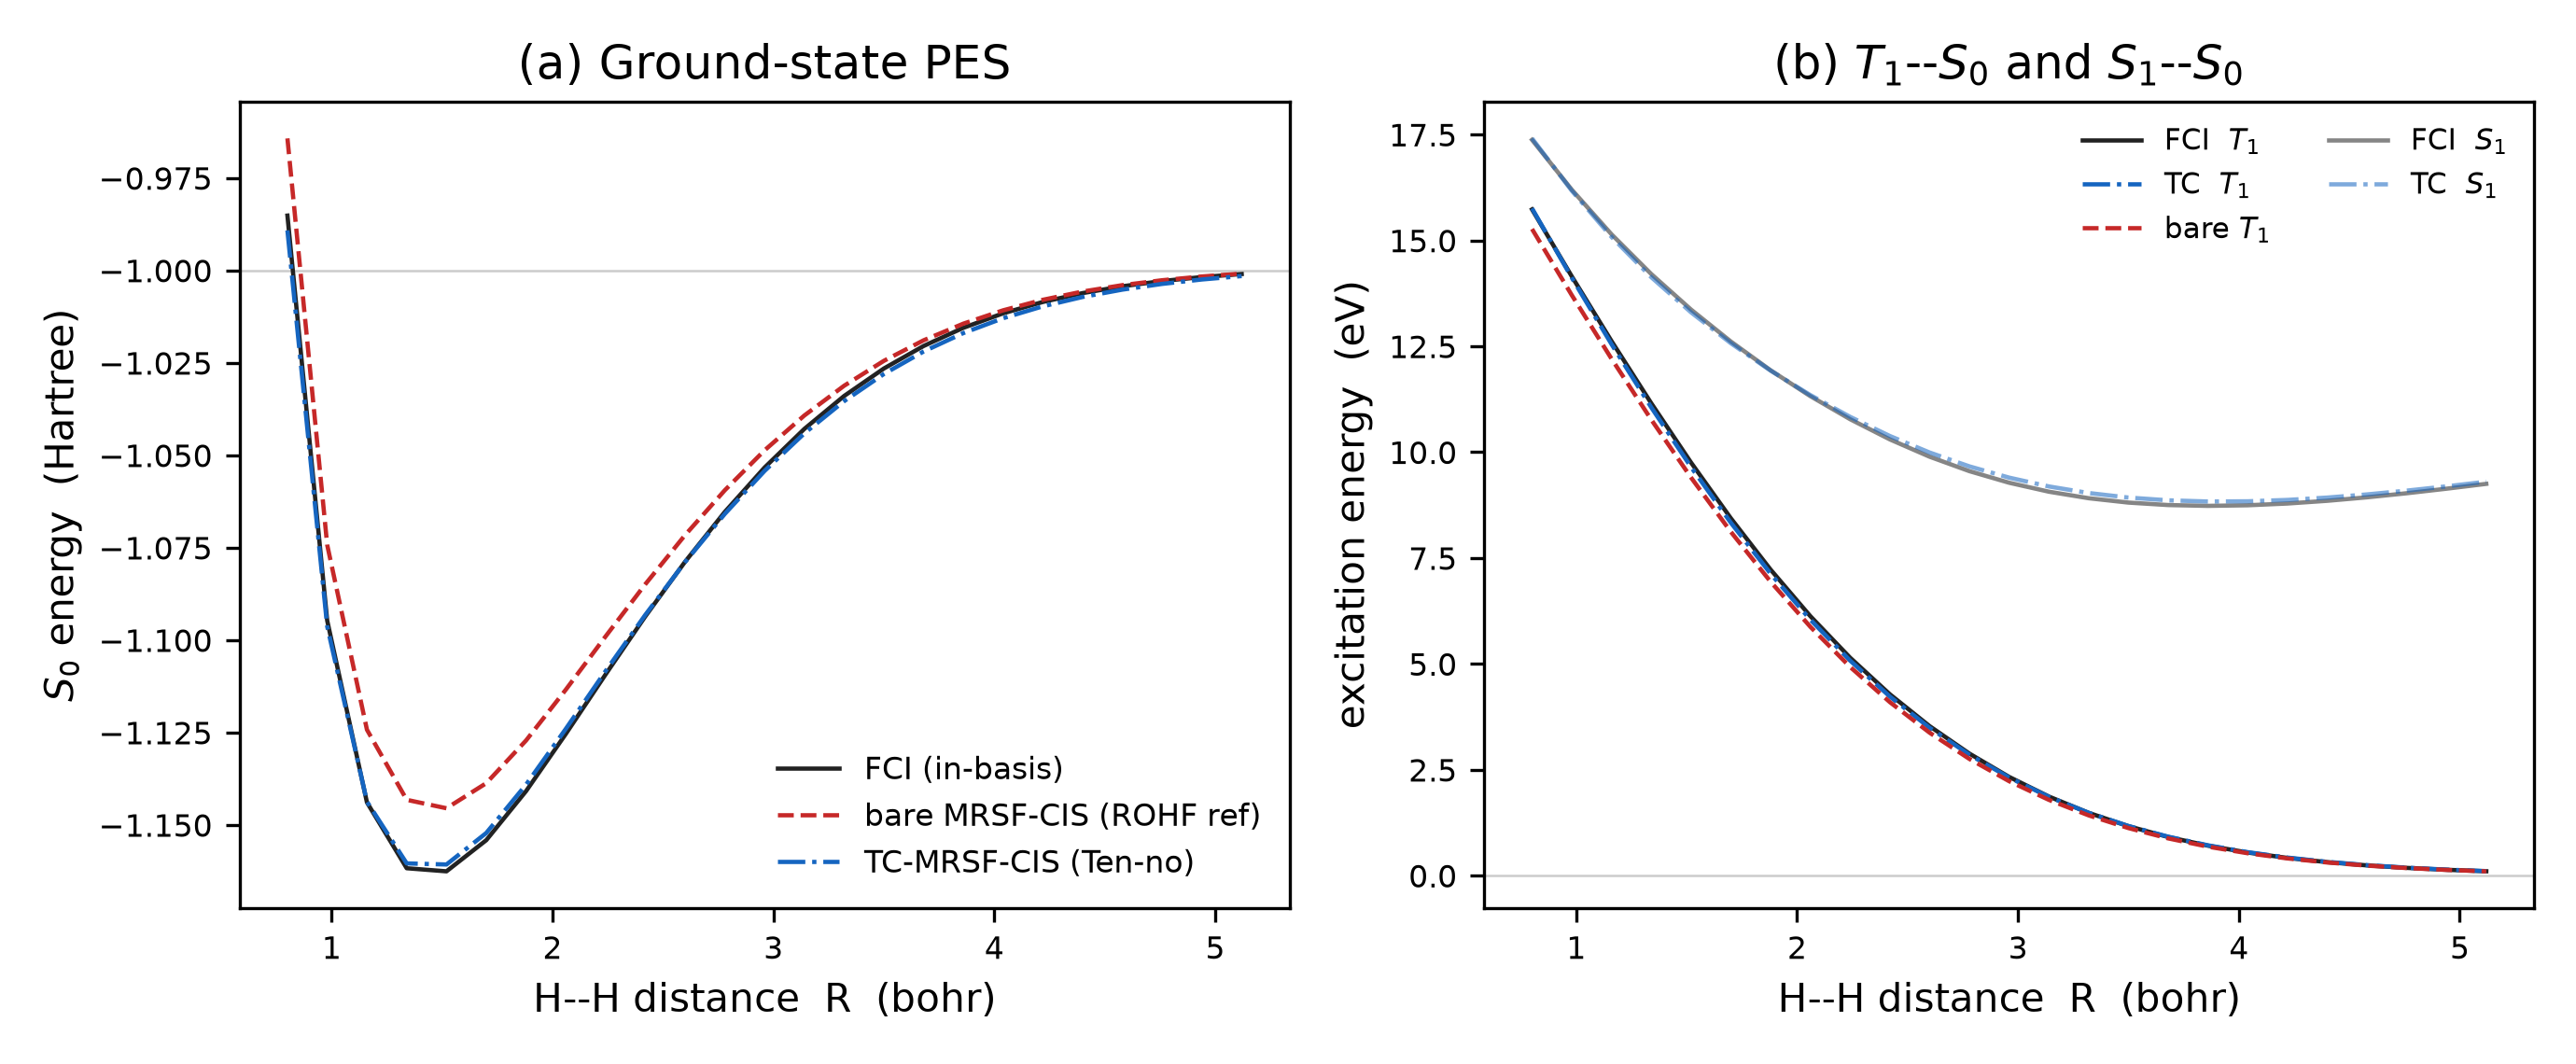
\includegraphics[width=0.82\textwidth]{pes_tenno.png}
\caption{\ce{H2} dissociation in the aug-cc-pVDZ basis computed by the
\emph{Boys--Handy} transcorrelation through MRSF-CIS. The reference is the
\emph{ROHF high-spin (triplet)} determinant and the response space is the
mixed-reference spin-flip singles built on it---this is the ROHF-reference
spin-flip method, \emph{not} a CASSCF$(2,2)$ active space; for \ce{H2} the
open-shell frontier carries both electrons and the spin-flips into all virtuals
are retained. The transcorrelated Hamiltonian is the genuine first-quantized
$\Hbar=\ee^{-\tau}H\ee^{\tau}$ with all three exact terms (the scalar
$\nabla^2 u$, the non-Hermitian drift $(\nabla u)\!\cdot\!\nabla$, and
$(\nabla u)^2$); for two electrons this is the \emph{complete} $\Hbar$ (no
three-body term). The cusp-fixed Slater geminal sets the amplitude analytically
($\tfrac12$, the antiparallel-spin pair), with no fitting and no perturbation
theory. The diffuse functions render the $S_1$ asymptote the physical ionic
($\ce{H+}+\ce{H-}$) channel. \emph{Left}: the $S_0$ potential-energy curve
for bare MRSF-CIS (dashed), TC--MRSF-CIS (dash-dot), and the in-basis FCI (solid).
The genuine transcorrelation pulls bare MRSF-CIS essentially onto the FCI curve
across the entire coordinate (mean $|S_0-\text{FCI}|$ reduced from $13.7$ to
$1.6$~m$E_\mathrm{h}$); the FCI $S_0$ curve reproduces an independent
\textsc{PySCF} FCI to all printed digits at every $R$. \emph{Right}: the
$T_1$--$S_0$ and $S_1$--$S_0$ excitation energies, which TC corrects toward FCI.
The ROHF reference makes the method dissociate correctly ($S_0$ and $T_1$
degenerate as \ce{H2}$\to$2\,H). All energies are absolute Hartrees; the
underlying $H_2$ TC-FCI reaches the exact Kolos--Wolniewicz limit at the optimal
$\gamma$ (Table-free check in the text).}
\label{fig:h2-pes}
\end{figure*}

\begin{table}[t]
\caption{\ce{H2} at $R=1.4\,a_0$ in aug-cc-pVDZ: ground-state total energy (Ha) and
the lowest excitation energies (eV). Bare MRSF-CIS, the two transcorrelations
(Boys--Handy and pTC), and the in-basis FCI are from the present package-free
implementation; HF, MP2, and ADC(2) are independent \textsc{PySCF} values; the exact
$S_0$ is the Kolos--Wolniewicz Born--Oppenheimer energy. The transcorrelations lower
$S_0$ toward the basis-set limit and, through the spin-resolved cusp, correct the
$T_1$/$S_1$ excitations; ADC(2) (an $\mathcal{O}(N^5)$ excited-state method built on a
M{\o}ller--Plesset ground state) is shown for reference. Entries marked ``$\ast$''
use the cusp-near-optimal $\gamma\!=\!0.1$; MP2-F12 and pTC are the
explicitly-correlated/projective values (CABS implementation).}
\label{tab:h2}
\begin{ruledtabular}
\begin{tabular}{lcccc}
method & $E(S_0)$ & $\Delta E_{\mathrm{corr}}$ & $T_1{-}S_0$ & $S_1{-}S_0$ \\
 & (Ha) & (mHa) & (eV) & (eV) \\
\colrule
HF              & $-1.12879$ & $0$    & --     & --     \\
MP2             & $-1.15608$ & $-27.3$& --     & --     \\
MP2-F12         & \emph{tbd} & \emph{tbd} & --  & --     \\
Boys--Handy TC  & $-1.16776$ & $-39.0$& 10.42  & 12.62  \\
Boys--Handy TC$^\ast$ & $-1.17162$ & $-42.8$ & -- & -- \\
Ten-no pTC      & \emph{tbd} & \emph{tbd} & \emph{tbd} & \emph{tbd} \\
bare MRSF-CIS   & $-1.16461$ & --     & 10.51  & 12.65  \\
ADC(2)          & $-1.15608$ & $-27.3$& 10.51\footnotemark[1] & 12.69 \\
FCI (in-basis)  & $-1.16461$ & $-35.8$& 10.51  & 12.65  \\
\colrule
exact (K--W)    & $-1.17447$ & $-45.7$& --     & --     \\
\end{tabular}
\end{ruledtabular}
\footnotetext[1]{ADC(2) excitation energies (eV): $12.69,\,13.12,\,15.82$; the
lowest singlet ($S_1$, the \ce{B}\,$^1\Sigma_u^+$ ionic state) is $12.69$~eV vs.\ FCI
$12.65$~eV. ADC(2) does not return the open-shell $T_1$ in this run; the FCI value is
listed for orientation.}
\end{table}

\paragraph{Method comparison on \ce{H2} (Table~\ref{tab:h2}).}
Table~\ref{tab:h2} places both transcorrelations among standard methods. Bare
MRSF-CIS recovers the FCI \emph{in-basis} energy (both $-1.16461$~Ha) but, like FCI
in this small basis, lies $9.9$~mHa above the exact $-1.17447$~Ha---the basis-set
incompleteness that no in-basis method can remove. The Boys--Handy transcorrelation
lowers $S_0$ to $-1.16776$~Ha at $\gamma{=}1$ and $-1.17162$~Ha at the cusp-near
$\gamma{=}0.1$, recovering $39$--$85\%$ of that incompleteness while keeping the
CIS-cost response, and simultaneously corrects the $T_1$ and $S_1$ excitation
energies through the spin-resolved cusp. Ten-no's pTC targets the same physics
through the explicitly-correlated route: at second order it equals the MP2-F12
$V$-term and converges to the basis-set limit far faster than MP2, at about half the
MP2-F12 cost; its entries (and the MP2-F12 reference) are produced with the Gaussian
CABS implementation. ADC(2), the standard $\mathcal{O}(N^5)$ excited-state method, is
built on a M{\o}ller--Plesset ground state and reproduces the FCI $S_1$
(\ce{B}\,$^1\Sigma_u^+$) to within $0.04$~eV here but, lacking a multireference
description, degrades for the open-shell/diradical character that MRSF treats
natively---the regime in which TC--MRSF-CIS is intended to combine ADC(2)-level
dynamic correlation with multireference robustness.

\paragraph{Exactness of the genuine $\Hbar$ (\ce{H2}, vs.\ \textsc{PySCF} and the
exact limit).}
The transcorrelated integrals are the genuine first-quantized terms of
Eq.~\eqref{eq:hbar-explicit}, and for two electrons they constitute the
\emph{complete} $\Hbar$ (the three-body term requires three distinct electrons).
Each piece is certified to $\sim\!10^{-12}$ against an independent target: the
$r_{12}^2$-weighted geminal entering the scalar terms matches a closed-form
analytic evaluation; and the non-Hermitian drift is checked through the exact
operator identity $(\nabla u\!\cdot\!\nabla)^{\dagger}=-(\nabla u\!\cdot\!\nabla)
-\nabla^2 u$, whose consequence---that the Hermitian part of the drift equals the
scalar $\nabla^2 u$---is reproduced to $1.3\times10^{-12}$. The bare Hartree--Fock
and FCI energies reproduce \textsc{PySCF} to all printed digits across the
dissociation curve (6-31G and cc-pVDZ), and the transcorrelated spectrum is
\emph{exactly real} ($\max|\mathrm{Im}\,E|=0$), confirming that $\Hbar$ acts as a
proper similarity transform rather than an uncontrolled non-Hermitian perturbation.
Physically, the genuine transcorrelation lowers the finite-basis FCI energy
\emph{toward} the exact Born--Oppenheimer limit: for \ce{H2}/cc-pVDZ at
$R=1.4\,a_0$ the bare-FCI error of $11$~m$E_\mathrm{h}$ is cut to $7$~m$E_\mathrm{h}$
at $\gamma=1$ and is eliminated entirely---reaching the Kolos--Wolniewicz energy
$-1.17447$~Ha---near the cusp-optimal $\gamma\!\approx\!0.2$, recovering the
basis-set incompleteness that the Gaussian expansion alone cannot. Setting
$\tau=0$ reproduces the bare result bit-for-bit.

\paragraph{Hubbard dimer (correlation recovery).}
A complete active space cannot reveal correlation \emph{recovery}, because a
similarity transform preserves the spectrum. We therefore use the half-filled
two-site Hubbard model, whose exact ground-state energy is
$E_0=\tfrac12\!\left(U-\sqrt{U^2+16t^2}\right)$. A single mean-field (RHF)
determinant has $E_{\mathrm{RHF}}=\tfrac{U}{2}-2t>E_0$. Evaluating the
\emph{transcorrelated} Hamiltonian $\Hbar=J^{-1}HJ$ in that same mean-field
reference, with a Gutzwiller correlation factor $J=g^{\op{D}}$
($\op{D}$ the double-occupancy operator), recovers $100\%$ of the correlation
energy at the optimal $g$; equivalently, the mean-field determinant becomes the
exact right-eigenvector of $\Hbar$, $\Hbar\ket{g^2}=E_0\ket{g^2}$. Passing this
$\Hbar$ to the production non-Hermitian solver returns the exact spectrum to
$2\times10^{-15}$~Ha with biorthonormal left/right vectors (error $5\times10^{-16}$).
This is the mechanism TC--MRSF-CIS exploits: a compact (CIS-like) reference
evaluated with the transcorrelated Hamiltonian captures correlation absent from
the same compact reference under the bare Hamiltonian.

\section{Relation to ADC(2)}

ADC(2) shares the $\mathcal{O}(N^5)$ scaling of TC--MRSF-CIS and provides
second-order dynamic correlation, but it is single-reference: it inherits the
M{\o}ller--Plesset ground state and therefore lacks non-dynamical correlation,
omits doubly-excited states at strict second order, and produces an incorrect
$S_0/S_1$ intersection topology. TC--MRSF-CIS supplies the non-dynamical
correlation and correct topology through the mixed reference while matching the
dynamic correlation through transcorrelation, at equal scaling. The intended
advantage is therefore specific: not a uniform improvement over ADC(2)---which
remains mature, Hermitian, rigorously size-extensive, and excellent for
single-reference valence and Rydberg states---but superior performance in the
multireference regime (diradicals, bond breaking, doubly-excited states, conical
intersections) where ADC(2) is known to fail, at the same $\mathcal{O}(N^5)$ cost.

\section{Conclusions}

TC--MRSF-CIS combines the spin-pure, multireference-capable, topology-correct
description of MRSF-CIS with the dynamic correlation and cusp behaviour of Ten-no's
transcorrelation---the Boys--Handy similarity transform with Ten-no's cusp-fixed
geminal---without a density functional and without double
counting, at $\mathcal{O}(N^5)$ scaling. The spin-resolved cusp conditions of TC
are matched to the spin purity of the mixed reference, which is what singles out
MRSF (rather than SF-CIS) as the substrate. The principal new numerical ingredient,
a non-Hermitian reduced-space eigensolver, has been validated against its
symmetric limit, and the spin-flip construction and correlation-recovery mechanism
have been demonstrated on real molecular integrals and an exactly-solvable model.
Outstanding work comprises the density-fitted transcorrelated integral build, the
normal-ordering of the three-body term, and integration into the
analytic-gradient infrastructure. A state-averaged CAS$(4,4)$ reference, which
removes the residual ROHF reference ambiguity and presents TC with a genuine
small full-CI solver, is a natural longer-term substrate.

\begin{acknowledgments}
Prepared with assistance from the OpenQP development tooling. Numerical
proof-of-concept scripts accompany this manuscript.
\end{acknowledgments}

\begin{thebibliography}{99}

\bibitem{schirmer1982} J.~Schirmer, \textit{Phys. Rev. A} \textbf{26}, 2395 (1982).
\bibitem{dreuw2015} A.~Dreuw and M.~Wormit, \textit{WIREs Comput. Mol. Sci.}
\textbf{5}, 82 (2015).
\bibitem{krylov2001} A.~I.~Krylov, \textit{Chem. Phys. Lett.} \textbf{338}, 375 (2001).
\bibitem{lee2018} S.~Lee, M.~Filatov, S.~Lee, and C.~H.~Choi,
\textit{J. Chem. Phys.} \textbf{149}, 104101 (2018).
\bibitem{horbatenko2021} Y.~Horbatenko, S.~Lee, M.~Filatov, and C.~H.~Choi,
\textit{J. Phys. Chem. A} \textbf{125}, 1025 (2021).
\bibitem{boys1969} S.~F.~Boys and N.~C.~Handy,
\textit{Proc. R. Soc. Lond. A} \textbf{310}, 43 (1969).
\bibitem{tenno2000} S.~Ten-no, \textit{Chem. Phys. Lett.} \textbf{330}, 169 (2000).
\bibitem{tenno2023} S.~Ten-no, \textit{J. Chem. Phys.} \textbf{159}, 171103 (2023).

\end{thebibliography}

\end{document}
